% Please do not change the document class
\documentclass{scrartcl}

% Please do not change these packages
\usepackage[hidelinks]{hyperref}
\usepackage[none]{hyphenat}
\usepackage{setspace}
\doublespace

% You may add additional packages here
\usepackage{amsmath}

% Please include a clear, concise, and descriptive title
\title{Your Title Here}

% Please do not change the subtitle
\subtitle{COMP230 - Ethics and Professionalism}

% Please put your student number in the author field
\author{1702208}

\begin{document}

\maketitle

\section{Introduction}

Nowadays video games have become a very common way of spending time among adolescents and adults. Although playing games have both negative and positive effects. Positive effects are usually stress reduction\cite{russoniello2009effectiveness}, relaxation\cite{wack2009relationships}, emotional disturbances in children\cite{jones2014gaming}\cite{hull2009computer} and a lot more. But there are still some negative consequences. Besides the most common - addiction - there are aggression, antisocial behaviour and violence, that usually depends on the game itself. But in this paper, main focus will be set on addiction, which requires further learning. 

\section{Skinner box}

Some games are intentionally designed to be addictive. That way they are putting players into a digital Skinner box. So-called Skinner box, also called an operant conditioning chamber \cite{skinnerbox}, was developed by Burrhus Frederic Skinner - ``American psychologist and an influential exponent of behaviourism"\cite{bfskinner}. He was studying human behaviour ``in terms of responses to environmental stimuli"\cite{bfskinner}. His Skinner box metaphor is related to players being addictive to a certain game whether they want that or not. 

This experiment was based on a laboratory rat, or other small animal, being put in a small glass box equipped with drinking tubes, food pellets and a bar or key that can be pressed\cite{skinnerbox}\cite{nyskinnerbox}. First, it was given a food pellet by looking at the lever, after - getting close to it and, eventually, pressing the lever. But not every press would give a food pellet, which made the rat press the lever continuously to sometimes get its reward. Moreover, some presses could dispense an unpleasant reinforce. For example, lights, sounds or images or, in the worst case, the floor may be electrified\cite{skinnerbox}.

This experiment relates to human behaviour as well. This is very well shown in games when designers intend to reward player for their continuous efforts, but rewards are not always satisfying for players or there are no reward at all. This stimulates them play more and more to eventually get that reward and therefore get closer to achieving one's personal goal.

\section{Player's fault or developers' intentions?}

Addictive games are usually most of the Massive Multi-player Online Role Playing Games (MMORPGs), Competitive games and casual/mobile games. Casual games are designed to give us satisfaction for a minimal input\cite{vgaddiction}. Whereas MMORPGs and competitive games stimulate us to play more and more of these games by levelling up or constantly getting better at the game. It generates previously mentioned digital Skinner box. Player are always looking for a rewards and therefore continuing to play this game in hope of getting better gear and levelling up. This is shown in picture \ref{fig:comic} in a comic way. Nevertheless, it's very accurate about most MMORPGs.

\begin{figure}
  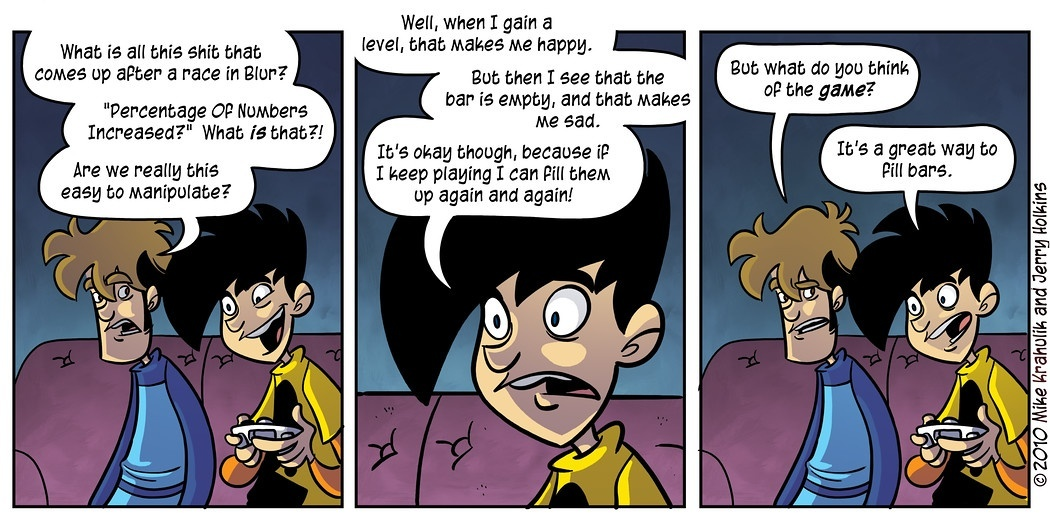
\includegraphics[width=\linewidth]{Images/AddictionComic.jpg}
  \caption{Addiction comic.}
  \label{fig:comic}
\end{figure}

Free-to-play games can also be addictive by being designed to ``monetize the seven deadly sins"\cite{vgaddiction}. This means having better gear, being higher level, wanting that in-game item, getting that in-game consumable, speeding up grinding, getting a revenge on a player, looking cooler than others - and every single one of these require paying real money. 

\section{Third Key Skill}

Write about 200 words. As above.

\section{Fourth Key Skill}

Write about 200 words. As above.

\section{Fifth Key Skill}

Write about 200 words. As above.

\section{Conclusion}

Write your conclusion here. Though the conclusion should be brief, no more than 100 words, it should do more than merely summarise the report. Focus on the five SMART actions that you intend to take in order to overcome any challenges and/or obstacles. Contextualise how this will help you towards your intended career goal and how this may improve your project for the next semester.

\bibliographystyle{ieeetran}
\bibliography{references}

\end{document}